\recipe{Sourdough}
\makes{Makes one medium loaf}
\worktime{30 minutes}
\totaltime{4 hours}
\source{}

\begin{ingredients}
    \item Strong white flour, \SI{400}{\gram}
    \item Whole wheat flour, \SI{100}{\gram}
    \item Water, \SI{370}{\gram}
    \item Sourdough starter, \SI{100}{\gram}
    \item Salt, \SI{7}{\gram}
\end{ingredients}

\begin{method}
Mix starter, flour, and water. Rest for around \SI{1}{\hour}.

Stretch and fold the dough a couple of times. Then rest dough for \SI{30}{\minute}. Repeat this 4 times.

Stretch and fold into a ball. Place in a floured napkin in a bowl (rice flour works well) and place in the fridge for \SI{12}{\hour} to \SI{24}{\hour}.
    
Preheat oven to \temp{220} and place a baking-paper-lined Dutch oven or glass bowl into the oven to warm up.
    
Transfer dough to the Dutch oven or bowl and bake for \SI{30}{\minute} covered.

Reduce oven temperature to \temp{200} and remove lid for another \SI{15}{\minute}.

Remove bread from oven and rest for \SI{30}{\minute} before serving.
\end{method}




\begin{figure}[h]
  	\centering
  	
  	\begin{tikzpicture}
  		% Save the image in a box to get its dimensions
  		\sbox0{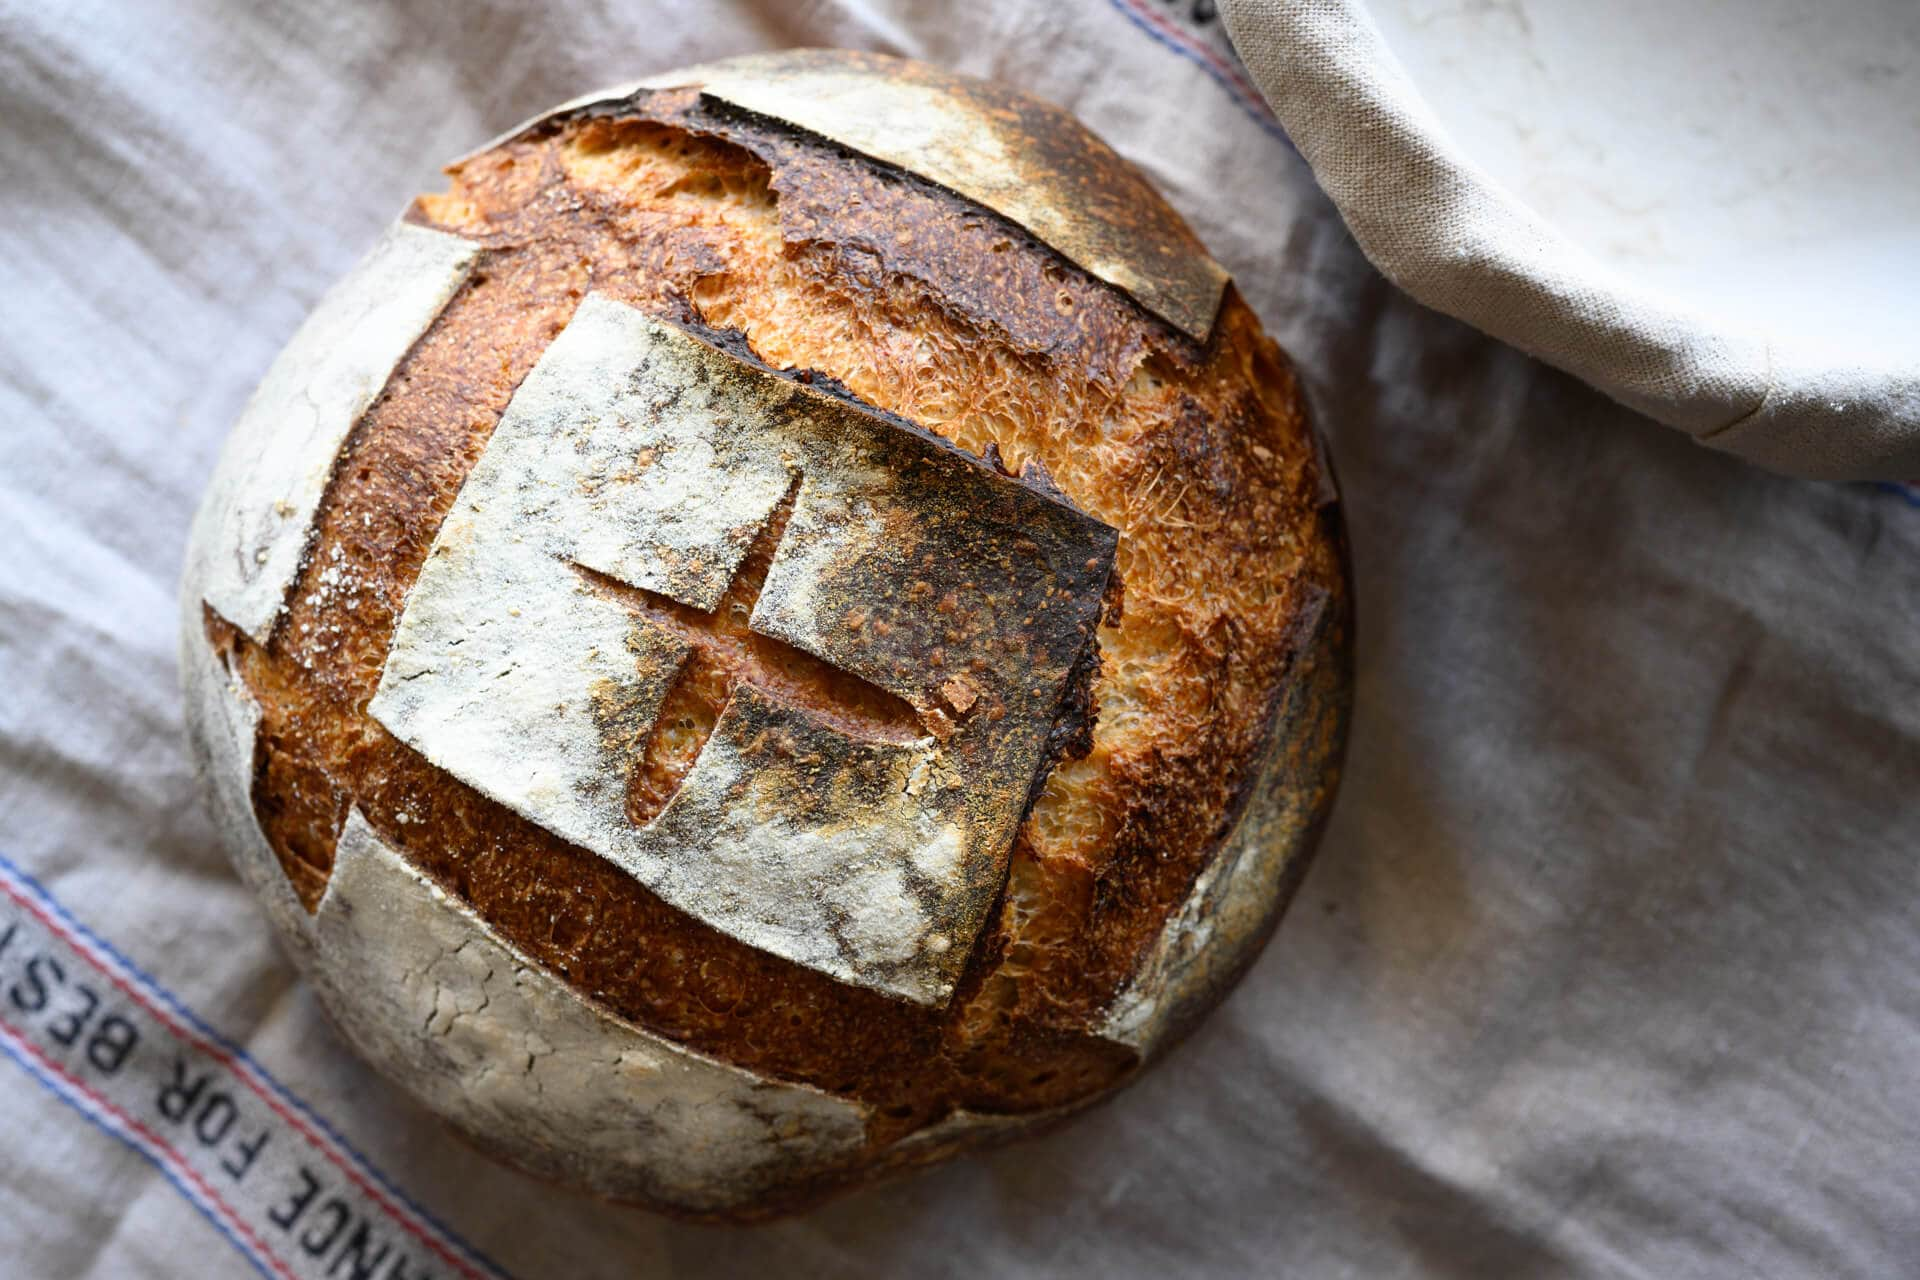
\includegraphics[width=\linewidth]{images/theperfectloaf-a-simple-workweek-sourdough-bread-recipe-1.jpg}}%
  
  		% Draw a clipping rectangle with rounded corners
  		\path[clip, rounded corners=0.5cm] (0,0) rectangle (\wd0,\ht0);
  
  		% Place the image inside the clipped area
  		\node[inner sep=0pt, outer sep=0pt, anchor=south west] at (0,0) {\usebox0};
	\end{tikzpicture}

  \caption*{}
\end{figure}
    
